\smalltitle{سوال 1}

\noindent
\textbf{الف)}

در ابتدا حالت کلی مدار را رسم می‌کنیم
(بدون $N$ و $Z$):

\begin{figure}[H]
    \centering
    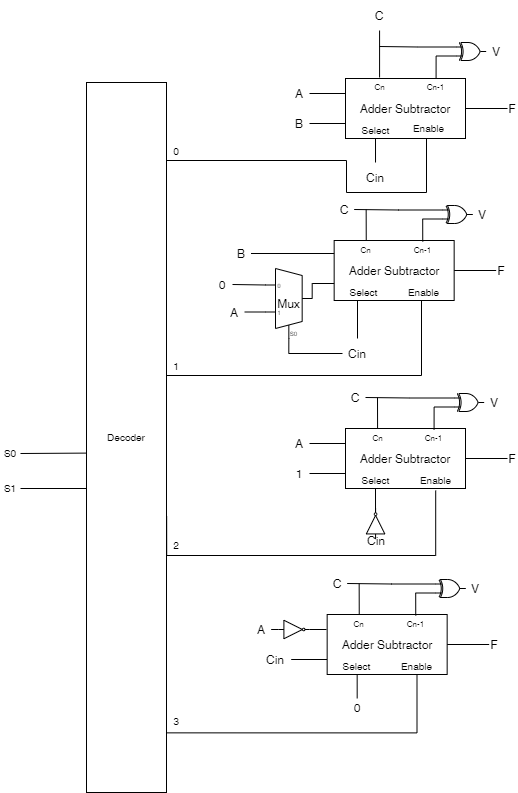
\includegraphics[scale=0.5]{source/1-1.png}
    \caption{مدار کلی \lr{ALU}}
    \label{1-1-circuit}
\end{figure}

حال باید ببینیم که
$N$
و
$Z$
را چه طور باید تشخیص دهیم. برای
$Z$
باید تمامی بیت‌ها را
$NOR$
کنیم و برای
$N$
باید تنها باید بیت آخر
$F$
را برگردانیم.

\noindent
\textbf{ب)}

\begin{enumerate}
    \item \lr{BHI}: برای چک کردن بیشتر بودن کافی است که چک کنیم که جواب نه 0 باشد و نه carry داشته باشد.
    \item \lr{BHE}: دقیقا مثل \lr{BHI} است ولی چک کردن $Z$ لازم نیست.
    \item \lr{BLO}: دقیقا نقیض نتیجه‌ی \lr{BHE}
    \item \lr{BLOE}: دقیقا نقیض نتیجه‌ی \lr{BHI}
    \item \lr{BE}: کافی است که چک کنیم که $Z$ برابر صفر باشد.
    \item \lr{BNE}: نقیض \lr{BE}
    \item \lr{BGT}: اول از همه اینکه اگر مثل \lr{BHI} فلگ $Z$ فعال باشد اعداد مساوی می‌‌شوند و باید صفر را برگردانیم.
    حال فرض کنید که جفت
    $N$ و $V$
    صفر باشند. نه \lr{overflow} رخ داده است و نه عدد منفی است پس $A > B$ است.
    همچنین اگر جفت آنها یک باشند بدین معنا است یعنی اینکه \lr{overflow} رخ داده. \lr{overflow} بدین دلیل رخ می‌دهد که تعداد بیت‌های رجیستر‌های ما جواب‌گو این تعداد رقم نیستند.
    پس در اصل حاصل تفریق ما مثبت بوده است و باز هم این موضوع نشان‌دهده‌ی این است که $A > B$ است.
    در صورتی که یکی از آنها مثبت باشد و یکی منفی بدین معنا است که عدد حاصل باید منفی می‌بوده و $A < B$ است.
    \item \lr{BGE}: دقیقا مثل \lr{BGT} ولی دیگر شرط $Z = 0$ را نداریم.
    \item \lr{BLT}: نقیض \lr{BGE}
    \item \lr{BLE}: نقیض \lr{BGT}
\end{enumerate}

\begin{figure}[H]
    \centering
    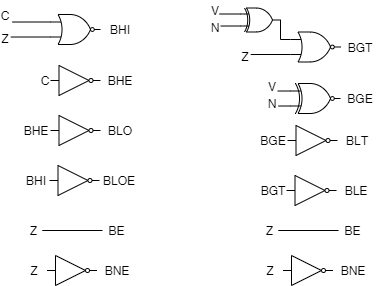
\includegraphics[scale=0.75]{source/1-2.png}
    \caption{گیت‌های مورد نیاز برای گرفتن نتیجه‌ی شرط}
    \label{1-2-circuit}
\end{figure}